%%%%%%%%%%%%%%%%%%%%%%%%%%%%%%%%%%%%%%%%%
% Large Colored Title Article
% LaTeX Template
% Version 1.1 (25/11/12)
%
% This template has been downloaded from:
% http://www.LaTeXTemplates.com
%
% Original author:
% Frits Wenneker (http://www.howtotex.com)
%
% License:
% CC BY-NC-SA 3.0 (http://creativecommons.org/licenses/by-nc-sa/3.0/)
%
%%%%%%%%%%%%%%%%%%%%%%%%%%%%%%%%%%%%%%%%%

%----------------------------------------------------------------------------------------
%	PACKAGES AND OTHER DOCUMENT CONFIGURATIONS
%----------------------------------------------------------------------------------------

\documentclass[DIV=calc, paper=a4, fontsize=11pt, twocolumn]{scrartcl}	 % A4 paper and 11pt font size
\usepackage{etex}
\usepackage{lipsum} % Used for inserting dummy 'Lorem ipsum' text into the template
\usepackage[english]{babel} % English language/hyphenation
\usepackage[protrusion=true,expansion=true]{microtype} % Better typography
\usepackage{amsmath,amsfonts,amsthm} % Math packages
\usepackage[svgnames]{xcolor} % Enabling colors by their 'svgnames'
\usepackage[hang, small,labelfont=bf,up,textfont=it,up]{caption} % Custom captions under/above floats in tables or figures
\usepackage{booktabs} % Horizontal rules in tables
\usepackage{fix-cm}	 % Custom font sizes - used for the initial letter in the document

\usepackage{algorithmic}
\usepackage{algorithm}
\usepackage{html}
\usepackage{slashbox} % table cell diagonal split
\usepackage{url}
\usepackage{graphicx}
\usepackage{wrapfig}
\usepackage{array}
\usepackage{longtable}
\usepackage{color}
\usepackage{microtype}    % improves, among other things, line-breaks in narrow columns
\usepackage{enumitem}
\usepackage{eucal}
\usepackage{tikz-qtree} 	% drawing hierarchies

\usepackage[disable]{todonotes} % To remove in-line review comments, use 'disable'
%\usepackage[colorinlistoftodos,textsize=normalsize,textwidth=1\marginparwidth]{todonotes} % To add in-line review comments

\usepackage{sectsty} % Enables custom section titles
\allsectionsfont{\usefont{OT1}{phv}{b}{n}} % Change the font of all section commands

\usepackage{fancyhdr} % Needed to define custom headers/footers
\pagestyle{fancy} % Enables the custom headers/footers
\usepackage{lastpage} % Used to determine the number of pages in the document (for "Page X of Total")

%\usepackage[disable]{todonotes} % To remove in-line review comments, use 'disable'
%\usepackage[colorinlistoftodos,textsize=normalsize,textwidth=1\marginparwidth]{todonotes} % To add in-line review comments

% Headers - all currently empty
\lhead{}
\chead{}
\rhead{}

% Footers
\lfoot{}
\cfoot{}
\rfoot{\footnotesize Page \thepage\ of \pageref{LastPage}} % "Page 1 of 2"

\renewcommand{\headrulewidth}{0.0pt} % No header rule
\renewcommand{\footrulewidth}{0.4pt} % Thin footer rule

\usepackage{lettrine} % Package to accentuate the first letter of the text
\newcommand{\initial}[1]{ % Defines the command and style for the first letter
\lettrine[lines=3,lhang=0.3,nindent=0em]{
\color{DarkGoldenrod}
{\textsf{#1}}}{}}

%%----------------------------------------------------------------------------------------
%%	TITLE SECTION
%%----------------------------------------------------------------------------------------
%
%\usepackage{titling} % Allows custom title configuration
%
%\newcommand{\HorRule}{\color{DarkGoldenrod} \rule{\linewidth}{1pt}} % Defines the gold horizontal rule around the title
%
%\pretitle{\vspace{-30pt} \begin{flushleft} \HorRule \fontsize{50}{50} \usefont{OT1}{phv}{b}{n} \color{DarkRed} \selectfont} % Horizontal rule before the title
%
%\title{Article Title} % Your article title
%
%\posttitle{\par\end{flushleft}\vskip 0.5em} % Whitespace under the title
%
%\preauthor{\begin{flushleft}\large \lineskip 0.5em \usefont{OT1}{phv}{b}{sl} \color{DarkRed}} % Author font configuration
%
%\author{John Smith, } % Your name
%
%\postauthor{\footnotesize \usefont{OT1}{phv}{m}{sl} \color{Black} % Configuration for the institution name
%University of California % Your institution
%
%\par\end{flushleft}\HorRule} % Horizontal rule after the title
%
%\date{} % Add a date here if you would like one to appear underneath the title block
%
%%----------------------------------------------------------------------------------------
 % One pager
%%%%%%%%%%%%%%%%%%%%%%%%%%%%%%%%%%%%%%%%%%
% Large Colored Title Article
% LaTeX Template
% Version 1.1 (25/11/12)
%
% This template has been downloaded from:
% http://www.LaTeXTemplates.com
%
% Original author:
% Frits Wenneker (http://www.howtotex.com)
%
% License:
% CC BY-NC-SA 3.0 (http://creativecommons.org/licenses/by-nc-sa/3.0/)
%
%%%%%%%%%%%%%%%%%%%%%%%%%%%%%%%%%%%%%%%%%

%----------------------------------------------------------------------------------------
%	PACKAGES AND OTHER DOCUMENT CONFIGURATIONS
%----------------------------------------------------------------------------------------

%\documentclass[DIV=calc, paper=a4, fontsize=11pt, twocolumn]{scrartcl}	 % A4 paper and 11pt font size
\documentclass[DIV=calc, paper=a4, fontsize=11pt, twocolumn]{scrreprt}
\usepackage[english]{babel} % English language/hyphenation
%\usepackage[protrusion=true,expansion=true]{microtype} % XeTex Problem
\usepackage{amsmath,amsfonts,amsthm} % Math packages
\usepackage[svgnames]{xcolor} % Enabling colors by their 'svgnames'
\usepackage[hang, small,labelfont=bf,up,textfont=it,up]{caption} % Custom captions under/above floats in tables or figures
\usepackage{booktabs} % Horizontal rules in tables
\usepackage{fix-cm}	 % Custom font sizes - used for the initial letter in the document
\usepackage{epigraph}
\setlength{\epigraphwidth}{0.8\linewidth}
\setlength{\epigraphrule}{0pt}
\renewcommand*{\textflush}{flushright}
\renewcommand*{\epigraphsize}{\normalsize\itshape}


\usepackage{algorithmic}
\usepackage{algorithm}
\usepackage{html}
\usepackage{slashbox} % table cell diagonal split
\usepackage{url}
\usepackage{graphicx}
\usepackage{wrapfig}
\usepackage{array}
\usepackage{longtable}
\usepackage{color}
\usepackage{enumitem}
\usepackage{eucal}
\usepackage{tikz-qtree} 	% drawing hierarchies


\usepackage[disable]{todonotes} % To remove in-line review comments, use 'disable'
%\usepackage[colorinlistoftodos,textsize=normalsize,textwidth=1\marginparwidth]{todonotes} % To add in-line review comments

\usepackage{sectsty} % Enables custom section titles
%\allsectionsfont{\usefont{OT1}{phv}{b}{n}} % Change the font of all section commands

\usepackage{fancyhdr} % Needed to define custom headers/footers
\pagestyle{fancy} % Enables the custom headers/footers
\usepackage{lastpage} % Used to determine the number of pages in the document (for "Page X of Total")


\lhead{}
\chead{}
\rhead{}


\lfoot{}
\cfoot{}
\rfoot{\footnotesize Page \thepage\ of \pageref{LastPage}} % "Page 1 of 2"

\renewcommand{\headrulewidth}{0.0pt} % No header rule
\renewcommand{\footrulewidth}{0.4pt} % Thin footer rule

\usepackage{lettrine} % Package to accentuate the first letter of the text
\newcommand{\initial}[1]{ % Defines the command and style for the first letter
\lettrine[lines=3,lhang=0.3,nindent=0em]{
\color{DarkGoldenrod}
{\textsf{#1}}}{}}

\usepackage{titling} % Allows custom title configuration
\newcommand{\HorRule}{\color{DarkGoldenrod} \rule{\linewidth}{1pt}} % Defines the gold horizontal rule around the title
\pretitle{\vspace{-70pt} \begin{flushleft} \HorRule \fontsize{20}{20} \usefont{OT1}{phv}{b}{n} \color{DarkRed} \selectfont} % Horizontal rule before the title

\title{Computing Midsurface} % Your article title

\posttitle{\par\end{flushleft}\vskip 0.25em} % Whitespace under the title
\preauthor{\begin{flushleft}\large \lineskip 0.5em \usefont{OT1}{phv}{b}{sl} \color{DarkRed}} % Author font configuration
\author{Yogesh Kulkarni\\} % Your name
\postauthor{\footnotesize \usefont{OT1}{phv}{m}{sl} \color{Black} % Configuration for the institution name
College of Engineering Pune, India % Your institution
\par\end{flushleft}\HorRule} % Horizontal rule after the title

\date{} % Add a date here if you would like one to appear underneath the title block

%----------------------------------------------------------------------------------------

\begin{document}

\maketitle

\section{Introduction}
At early stages of design, CAD parts are often \textbf{idealized} before analyzing them in CAE, to save on compute time and resources. Thin-walled parts are idealized to \textbf{Midsurface}, a surface running through the part, midway of the thickness.
\vskip 2mm
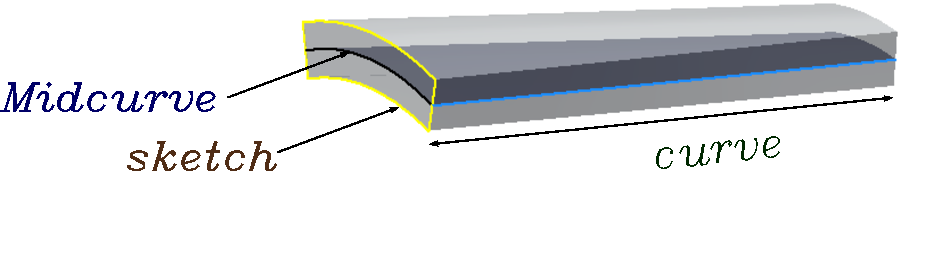
\includegraphics[width=0.7\linewidth]{../Common/images/MidsurfSmallProfile.pdf}
\vskip -2mm

Getting a connected Midsurface, {\em representing} the overall shape of the part, is still a challenging problem, due to non-deterministic/agreeable expected results and also complexity of the shapes. These problems are relatively less in simple shapes where one can imagine and expect accurate Midsurface and current algorithms are able to handle them. 

Typical approaches to compute Midsurface, in academics and commercial are:  Medial Axis Transform (MAT) and Medial Abstraction (MA).

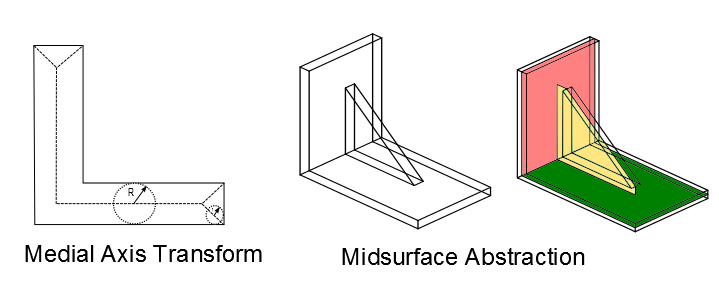
\includegraphics[width=0.8\linewidth]{../Common/images/MAT_Midsurf.png}

MAT suffers from extraneous branches and MA suffers from complexity in finding the face pairs.

Both approaches work on the final shape (Boundary representation - Brep) and thus find challenging to compute in case of complex surfaces, interactions etc. If this final shape is decomposed into smaller-simpler shapes, it would be easier and more deterministic to compute the Midsurface. Such decomposition is readily available in form of the \textbf{feature tree}.

\section{Approach [1]}
Many commercial CAD applications provide {\em Design-by-Features} approach. Part is built using features one-by-one in time-line order, almost in a Constructive-Solid-Geometry (CSG) like tree way. Leaves represent  Primitives/Tool-Bodies and internal nodes represent booleans. At each level of the tree, starting from first feature, shapes are simpler than the final shape. Boolean type is known. So computing Midsurface of the Tool-bodies and their boolean to the shape built till that level, is a more deterministic than detecting/computing Midsurface in the final shape.

\begin{itemize}[noitemsep,nolistsep]
\item Concurrently build Midsurface as the part gets created/updated. 
\item For each feature, compute Midsurface as below;
	\begin{itemize}[noitemsep,nolistsep]
	\item 2D Profiles: Generate \textbf{Midcurves} [2]
	\item Sweep based Features : Sweep \textbf{Midcurves} to generate Midsurface of the tool-body
	\item Boolean : Join tool-body-Midsurface with the Midsurface computed so far.
	\end{itemize}
\end{itemize}
%\centering 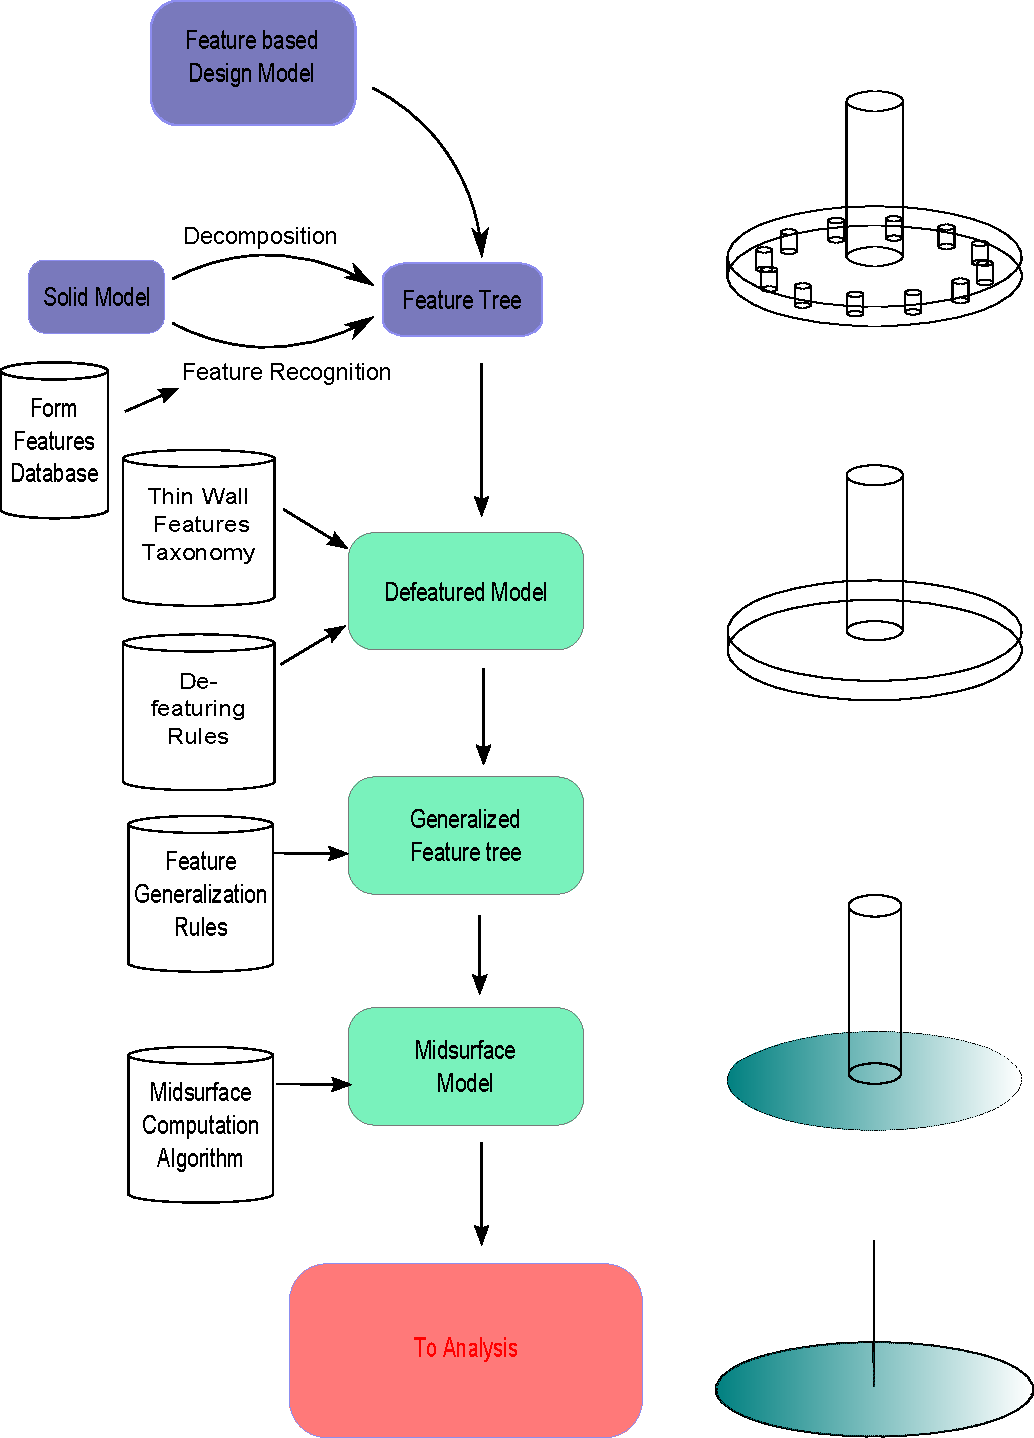
\includegraphics[height=0.7\linewidth]{../Common/images/SystemArchitecture.pdf}

%\section{De-featuring}
\section{Midcurve [2]}
\textbf{Goal}: Given a 2D profile (say, a closed polygon), how to compute the \textbf{Midcurve}.
\begin{itemize}[noitemsep,nolistsep]
\item Partition given shape into sub-shapes and then Midcurves can be generated for each eligible-simpler sub-polygon.
\item Later such individual Midcurves can be joined to form continuous Midcurves representing the original shape.
\end{itemize}
\vskip 2mm
\centering {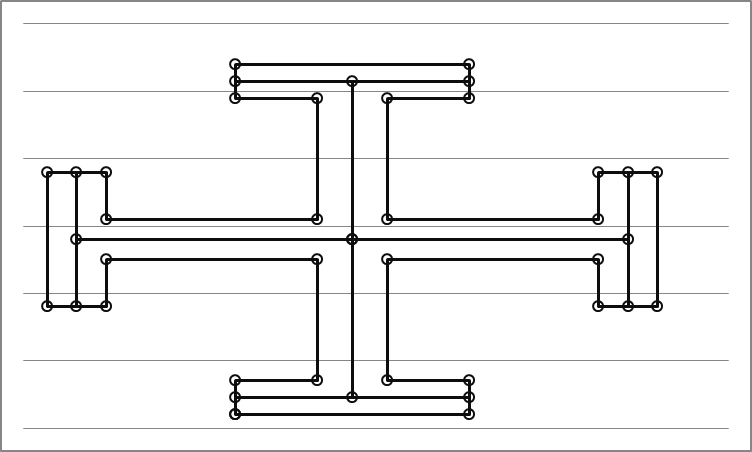
\includegraphics[scale=0.4]{../Common/images/Crossm.png}}

%\section{Midsurface}
\section{Papers}
\begin{enumerate}
\item Strategies for using feature information in model simplification, CAE Conf, IITM, 2013
\item Midcurves Generation Algorithm for Thin Polygons, ETES, Asansol, 2014
%\item \href{https://www.researchgate.net/profile/Yogesh_Kulkarni4/publication/259396573_Strategies_for_using_feature_information_in_model_simplification/file/60b7d52b695bc9cd8c.pdf?ev=pub_int_doc_dl&origin=publication_detail&inViewer=true}{Strategies for using feature information in model simplification}, CAE Conf, IITM, 2013
%\item \href{https://www.researchgate.net/profile/Yogesh_Kulkarni4/publication/259972281_Midcurves_Generation_Algorithm_for_Thin_Polygons/file/72e7e534148576285a.pdf?ev=pub_int_doc_dl&origin=publication_detail&inViewer=true}{Midcurves Generation Algorithm for Thin Polygons}, ETES, Asansol, 2014
\end{enumerate}
%\bibliographystyle{plain}
%\bibliography{../Common/Bibliography}
\end{document}